%!TEX root = main_ISMB.tex
\section{Results}
\label{sec:results}

\subsection{Implementation}
\label{sec:implementation}
Our software, \ourprog, was implemented in {\tt Python~2.7}. We used
\RNAinverse from the \textit{Vienna Package 2.0}~\cite{Hofacker:1994}.
All time benchmarks were run on a one AMD Opteron(tm) Processor 6278  at 2.4 GHz with cache of 512 KB.
 We used as parameter $\beta=15$, the penalty for an invalid base pair.



We present the average times spent by \ourprog and \RNAinverse to generate one sequence
with the required \GCContent in Figure~\ref{fig:time}. As expected, the time grows linearly
in function of the length of the structures for \ourprog.  A highly interesting feature
is the huge decrease in time of computation when there is $15\%$ free 
nucleotides inside the loops of the secondary structure.

\begin{figure}[ht!]
	\centering
	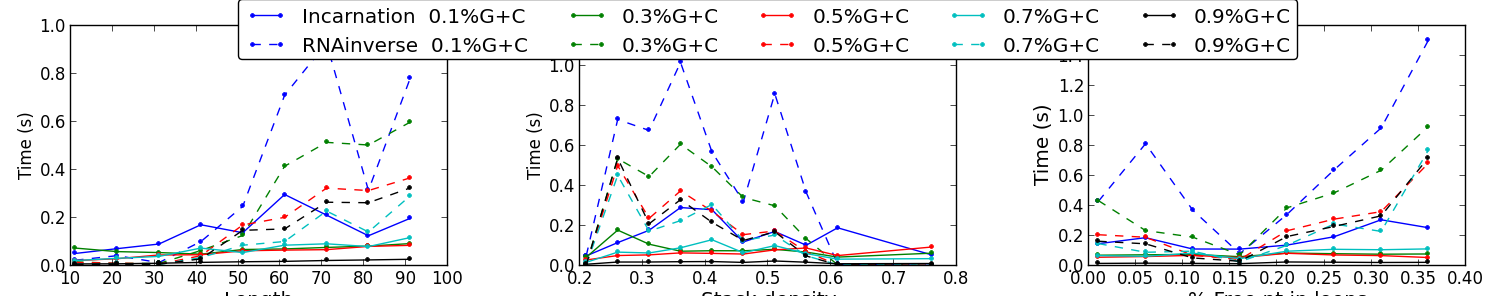
\includegraphics[width=\textwidth]{Figures/time_rnastrand_clustered_rnainverse_100samples_fix}
	\caption{Average time in seconds to generate one sequence. We explicitly show 
	the time spent by \ourprog (full line) and \texttt{RNAinverse} (dashed) for various \GCContent. The first plot is in function
	of the length of the structures. The second is in function of the stack
	density (i.e. $2\cdot\#stacks/length$) and the latter in function of 
	the proportion of free nucleotides (i.e. unpaired bases) within loops.}
	\label{fig:time}	
\end{figure}



\subsection{Dataset}
To evaluate the quality of our method, we used secondary
structures from the \RNASTRAND database~\cite{andronescu2008rna}.
Those are known secondary structure from a variety of organisms.
We select the same subset of $50$ structures as in~\cite{Levin:2012kx}, 
whose length ranges between $20$ and $100$ nucleotides. 

 To ease the visualization of the results, we clustered together strucures
 having similar length, stacks density and proportion of free-nucleotides in loops. 
  We present in Figure~\ref{fig:bins} the distribution of structures in each category.
 
 \begin{figure}[ht!]
 	\centering
	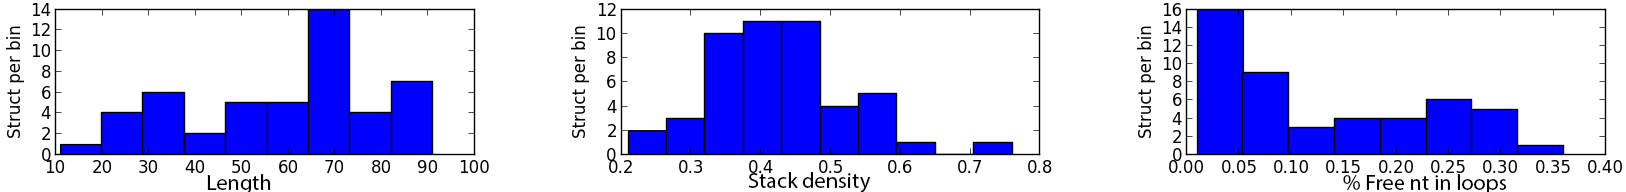
\includegraphics[width=\textwidth]{Figures/bins_distribution.png}
	\caption{Number of secondary structures per bin, according to our three clustering criteria.}
	\label{fig:bins}
 \end{figure}
 
 
\subsection{Design}
 To benchmark our method, we first started by sampling about $100$ sequences per structure. After correcting the free nucleotides with
 \texttt{RNAinverse} we computed their MFE with \texttt{RNAfold} from the \textit{Vienna Package 2.0}~\cite{Hofacker:1994}.
 
A first criterion is which percentage of sequences have as MFE the target
secondary structures. We are also interested by the number of structures
for which we can design at least one sequence with the desired MFE.
We show the results when using only \ourprog in 
 Figure~\ref{fig:mfe_struct_solved_noinverse}. As mentioned earlier, the high rate of failure
is due to the fact that no selection criterion is applied to
unpaired nucleotides. A local strategy is thus needed.
After processing \ourprog sequences with \RNAinverse to 
locally optimize the free nucleotides, we obtained the results 
shown in Figure~\ref{fig:mfe_struct_solved}. We observed
that length is, in general, not a good predictor for the hardness of designing a structure. 
Instead, a high number of free nucleotides in the structure seems to be a 
good measure of its design hardness. 
 The difficulty of 
designing sequences for targets with a high number of free nucleotides 
 in loops appears clearly in the last column of Figure~\ref{fig:mfe_struct_solved}.
Even with a \GCContent of $50\%$ and more, when at least
one solutions was found for almost all structures, most of the samples 
do not fold into the target. A few structures remained unsolved under
all \GCContent.


\begin{figure}[ht!]	
	\centering
	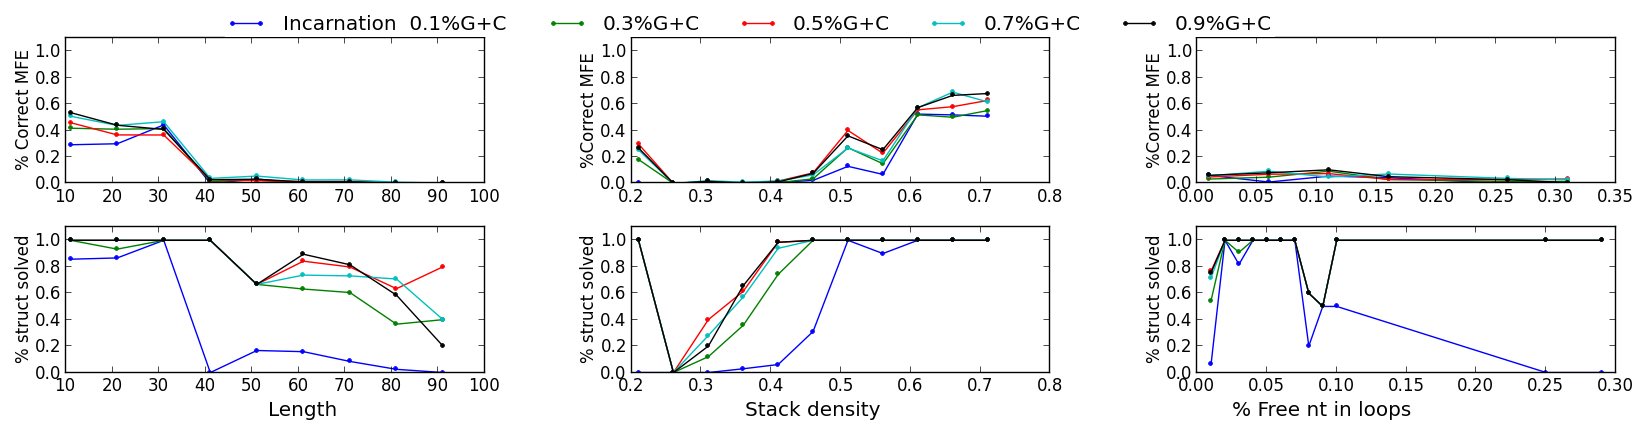
\includegraphics[width=\textwidth]{Figures/mfe_struct_solve_nornainverse.png}
	\caption{Quality of \ourprog results. The first row shows the percentage
	of sampled sequences folding into the target. The second shows the 	
	proportion	of structures for which at least one correct sequence was 
	sampled.}
	\label{fig:mfe_struct_solved_noinverse}	
\end{figure}



\begin{figure}[ht!]	
	\centering
	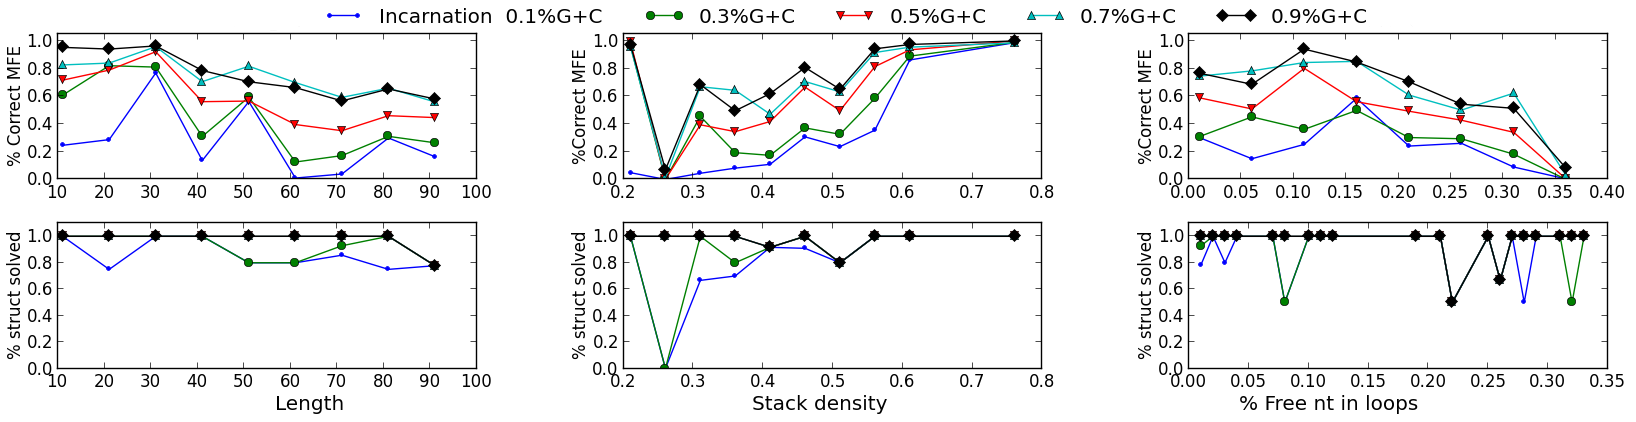
\includegraphics[width=\textwidth]{Figures/mfe_struct_solved}
	\caption{Quality of \texttt{Incarnation+RNAinverse} results. The first row shows the percentage
	of sampled sequences folding into the target. The second shows the 	
	proportion	of structures for which at least one correct sequence was 
	sampled.}
	\label{fig:mfe_struct_solved}	
\end{figure}
 
To evaluate the global quality of \ourprog sequences, we show
in Figure~\ref{fig:ss_sens} the ratio of well predicted base pairs in the
MFE structure of our sampled sequences. We can observe that, in all cases,
the hardest sequence to design are those with an extremely low \GCContent. As anticipated, those are the sequences with the weakest bonds.
We notice that the most accurate sequences yield a \GCContent
of $70\pm 10\%$. 

As discussed in Sec.~\ref{sec:implementation}, we notice a highly decreased
computational time needed to generate the sequences with $15\%$ free 
nucleotides in the loops. We remark that those structures also yield 
a much lower structural sensitivity.

\begin{figure}[ht!]
 	\centering
	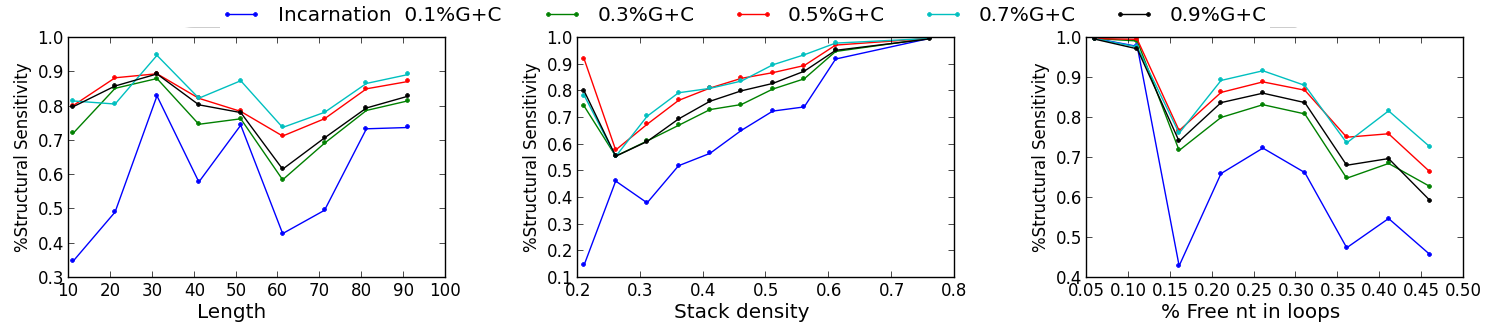
\includegraphics[scale=0.45]{Figures/rnastrand_clustered_rnainverse_100samples_struct_sens.png}
	\caption{Structural sensitivity (i.e. $\#$ well predicted base pairs / $\#$ base pairs in target) of the sampled sequences MFE. }
	\label{fig:ss_sens}	
\end{figure}


\subsection{Samples properties}

In this section, we further analyze the generated sequences that fold into the 
target structure. 

A desirable feature in sequence design, is to produce samples with a high
diversity. Figure~\ref{fig:nb_sols_entropy} shows the number of correct
solutions as their average entropy and base pair entropy, since 
\ourprog  only influences the distribution of nucleotides inside 
stacked base pairs. The most constraining factor for generating valid
 solutions seems to be  low \GCContent and the percentage of free nucleotides. Our method is able to generate 

Also, a critical properties in RNA sequence design is 
the frequency of the MFE. 
The sequence should be in its target conformation long enough to
perform the desired action. Presented in Figure~\ref{fig:freq} we see that
there is a slow decline of the frequency with the increase in size. Yet,
for an average \GCContent, the frequency stays over $10\%$ even
at size of $100$ nucleotides.


\begin{figure}[ht!]
	\centering
	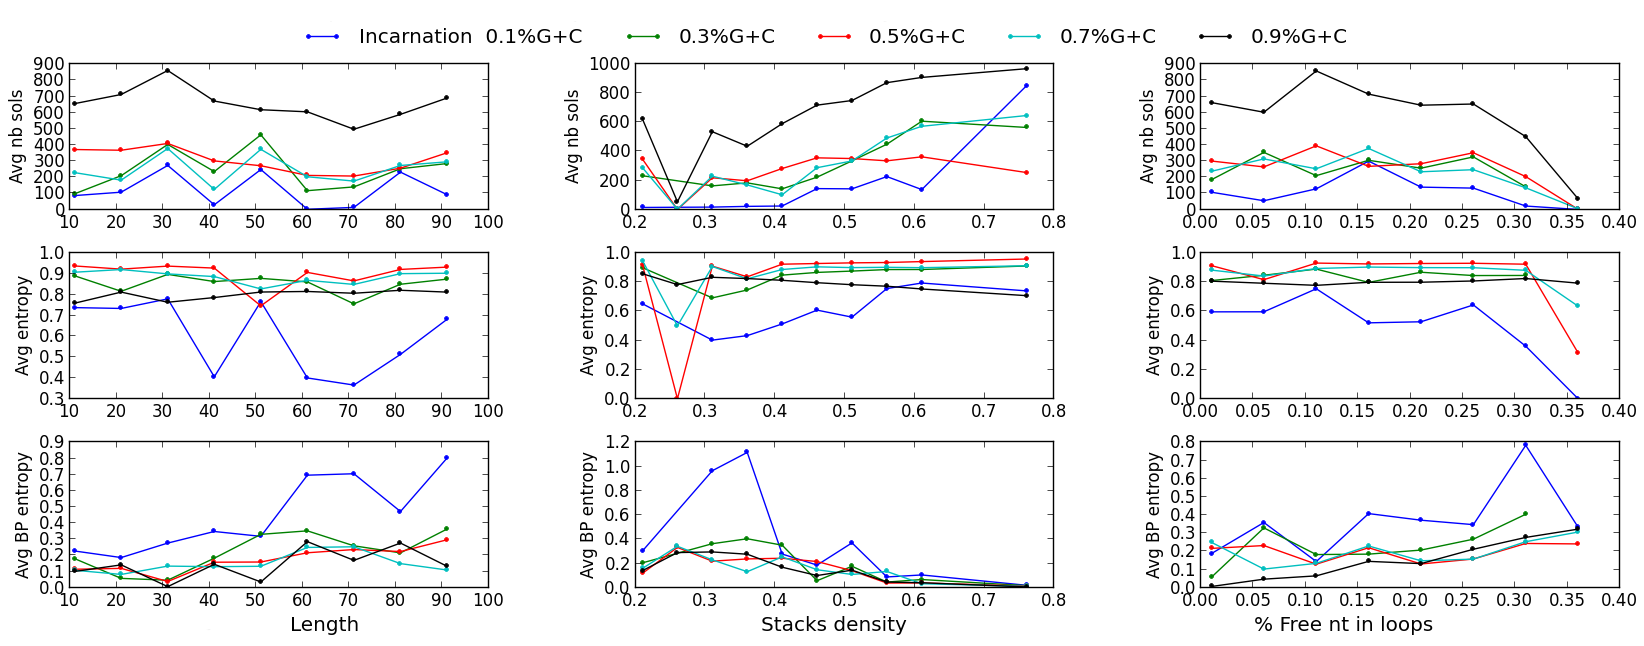
\includegraphics[width=\textwidth]{Figures/nb_sols_entropy.png}
	\caption{Number of solutions generated and their average entropy. 
	The last row presents only the entropy of the nucleotides inside base 
	pairs.}
	\label{fig:nb_sols_entropy}
\end{figure}



\begin{figure}[ht!]
	\centering
	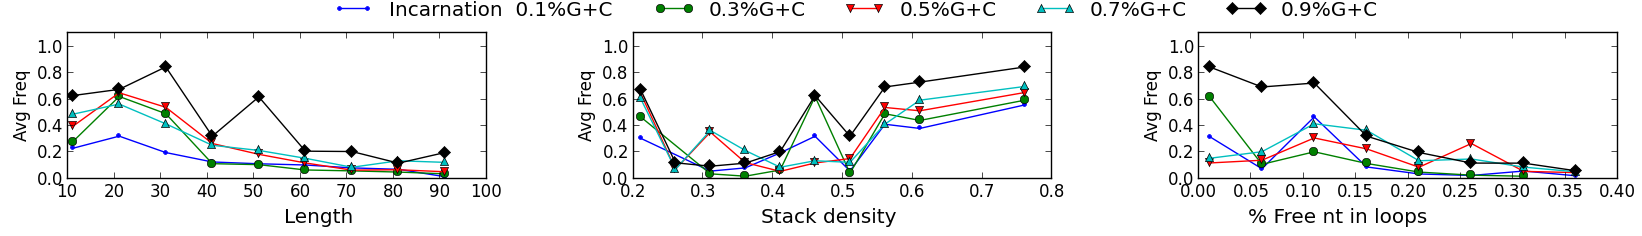
\includegraphics[width=\textwidth]{Figures/freq.png}
	\caption{Average frequency of the MFE.}
	\label{fig:freq}
\end{figure}

\subsection{Global sampling vs Local search vs Glocal approach}
<<<<<<< HEAD
Here, we are interested in estimating the impact of the design methodology on the performances. More precisely, we aim to determine the benefits of a global sampling approach (\ourprog), compared to both a glocal procedure (\ourprog + \RNAinverse) and a classical local search methodology (\RNAinverse). Thus, we compare our method to a pure local search procedure (see Section \ref{subsec:glocal_method}). Our results (See Fig. \ref{fig:rnainverse} in Supplementary data) show that \ourprog outperforms other strategies. In particular, the base pair entropy as well as diversity of sequences are favorable to \ourprog. This advantage is even more striking for low targeted \GCContent{}s regimes.
=======
Here, we are interested in estimating the impact of the design methodology on the performances. More precisely, we aim to what are the benefits of a global sampling approach (\ourprog), versus a glocal procedure (\ourprog + \RNAinverse) or the classical local search methodology (\RNAinverse). Thus, we compare our method to a pure local search procedure. In particular, here we compare to \RNAinverse as it is the program we used to do the local optimization (see Section \ref{subsec:glocal_method}). Our results (See Fig. \ref{fig:rnainverse} in Supplementary data) show that \ourprog overcome other strategies. In particular, the base pair entropy as well as diversity of sequences are favorable to \ourprog. This advantage is even more striking for low \GCContent regimes.
>>>>>>> bac85f3b6cf022d7b485ac16a605fafb9774b5b8

To complete this benchmark, we added the results obtained with the glocal procedure (\ourprog + \RNAinverse). We note that the results are slightly lower than those of \ourprog alone. However, we must stress that the \ourprog data consider only the sample of \ourprog already satisfying the MFE criterion. In fact \RNAinverse enable to ``correct'' a lot of sample sampled by \ourprog but without the good folding properties. Hence, our conclusion here is that the glocal approach \ourprog + \RNAinverse enable us to conserve the same level of performance but to drastically improve the success rate of our methodology. 






\label{fig:rnainverse}

